\documentclass[../defence.tex]{subfiles}

\begin{document}
  \begin{frame}{Wafer inhomogeneity - closed pore membranes wafer 296}
    \begin{columns}[onlytextwidth, T]
      \column{\dimexpr\linewidth / 21 * 10}
        \begin{block}{Isotherms}
          \tikzsetnextfilename{296_cp}
          \begin{tikzpicture}[scale=0.5, transform shape]
              \def\PrelMin{.87}
              \def\PrelMax{.945}
              \def\TransMin{1e-6}
              \def\TransMax{1}
              \def\LfMin{0}
              \def\LfMax{2}
              %
              \begin{axis}[
                /tikz/line join=bevel,
                grid,
                axis y line*=left,
                %legend style={at={(0,0.5)}, legend columns=2, anchor=north west},
                every axis plot,
                axis y line*=left,
                line width = 1pt,
                xmin = \PrelMin, xmax = \PrelMax,
                ymin = \LfMin, ymax = \LfMax,
                xlabel = {Relative pressure $P_\mathrm{rel}$},
                ylabel = {Liquid fraction $LF$},
                ytick = {0,0.25,0.50,0.75,1},
                ]
                % Add plots
                \addplot[mark=none, color=red] table [x=Prel,y=liquid_fraction]{tikz/graphs/wafer_inhomogeneities/296a_cond_2.txt};
                %\addlegendentry{$LF_\mathrm{cond}^\mathrm{296a}$}
                \addplot[mark=none, color=red!50] table [x=Prel,y=liquid_fraction]{tikz/graphs/wafer_inhomogeneities/296a_evap_2.txt};
                %\addlegendentry{$LF_\mathrm{evap}^\mathrm{296a}$}
                \addplot[mark=none, color=blue] table [x=Prel,y=liquid_fraction]{tikz/graphs/wafer_inhomogeneities/296b_cp_cond_1.txt};
                %\addlegendentry{$LF_\mathrm{cond}^\mathrm{296b}$}
                \addplot[mark=none, color=blue!50] table [x=Prel,y=liquid_fraction]{tikz/graphs/wafer_inhomogeneities/296b_cp_evap_1.txt};
                %\addlegendentry{$LF_\mathrm{evap}^\mathrm{296b}$}
                \addplot[mark=none, color=green] table [x=Prel,y=liquid_fraction]{tikz/graphs/wafer_inhomogeneities/296e_cond_2.txt};
                %\addlegendentry{$LF_\mathrm{cond}^\mathrm{296e'}$}
                \addplot[mark=none, color=green!50] table [x=Prel,y=liquid_fraction]{tikz/graphs/wafer_inhomogeneities/296e_evap_2.txt};
                %\addlegendentry{$LF_\mathrm{evap}^\mathrm{296e'}$}
                \addplot[mark=none, color=orange] table [x=Prel,y=liquid_fraction]{tikz/graphs/wafer_inhomogeneities/296f_cond_2.txt};
                %\addlegendentry{$LF_\mathrm{cond}^\mathrm{296f'}$}
                \addplot[mark=none, color=orange!50] table [x=Prel,y=liquid_fraction]{tikz/graphs/wafer_inhomogeneities/296f_evap_2.txt};
                %\addlegendentry{$LF_\mathrm{evap}^\mathrm{296f'}$}
              \end{axis}
              % transmission
              \begin{axis}[
                /tikz/line join=bevel,
                ymode=log,
                axis y line*=right, ylabel near ticks, yticklabel pos=right,
                line width = 1pt,
                xmin = \PrelMin, xmax = \PrelMax,
                ymin = \TransMin, ymax = \TransMax,
                ylabel = {Transmission $T$},
                xtick = {1e-1,1e-2,1e-3},
                ytick = {10,1,1e-1,1e-2,1e-3},
                ymajorgrids=true,
                %legend style={at={(0,0.5)}, legend columns=2, anchor=south west},
                ]
                % Add plots
                \addplot[mark=none, color=red] table [x=Prel,y=transmission]{tikz/graphs/wafer_inhomogeneities/296a_cond_2.txt};
                %\addlegendentry{$T_\mathrm{cond}^\mathrm{296a}$}
                \addplot[mark=none, color=red!50] table [x=Prel,y=transmission]{tikz/graphs/wafer_inhomogeneities/296a_evap_2.txt};
                %\addlegendentry{$T_\mathrm{evap}^\mathrm{296a}$}
                \addplot[mark=none, color=blue] table [x=Prel,y=transmission]{tikz/graphs/wafer_inhomogeneities/296b_cp_cond_1.txt};
                %\addlegendentry{$T_\mathrm{cond}^\mathrm{296b}$}
                \addplot[mark=none, color=blue!50] table [x=Prel,y=transmission]{tikz/graphs/wafer_inhomogeneities/296b_cp_evap_1.txt};
                %\addlegendentry{$T_\mathrm{evap}^\mathrm{296b}$}
                \addplot[mark=none, color=green] table [x=Prel,y=transmission]{tikz/graphs/wafer_inhomogeneities/296e_cond_2.txt};
                %\addlegendentry{$T_\mathrm{cond}^\mathrm{296e'}$}
                \addplot[mark=none, color=green!50] table [x=Prel,y=transmission]{tikz/graphs/wafer_inhomogeneities/296e_evap_2.txt};
                %\addlegendentry{$T_\mathrm{evap}^\mathrm{296e'}$}
                \addplot[mark=none, color=orange] table [x=Prel,y=transmission]{tikz/graphs/wafer_inhomogeneities/296f_cond_2.txt};
                %\addlegendentry{$T_\mathrm{cond}^\mathrm{296f'}$}
                \addplot[mark=none, color=orange!50] table [x=Prel,y=transmission]{tikz/graphs/wafer_inhomogeneities/296f_evap_2.txt};
                %\addlegendentry{$T_\mathrm{evap}^\mathrm{296f'}$}
              \end{axis}
          \end{tikzpicture}
        \end{block}
      \pause

      \column{\dimexpr\linewidth / 21}
      \column{\dimexpr\linewidth / 21 * 10}
        \begin{block}{Dry transmission mesurements}
          %\tikzsetnextfilename{wafer_296_transmission}
          \tikzexternaldisable
          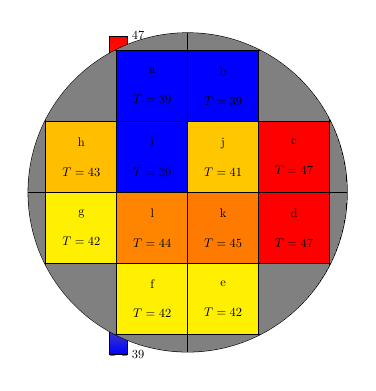
\begin{tikzpicture}[scale=0.45, transform shape]
            \begin{scope}[xshift=-2.5cm,yshift=-3cm]
              \begin{axis}[
                    hide axis,
                    colormap/hot,
                    xmin=-4.5, xmax=4.5,
                    ymin=-4.5, ymax=4.5,
                    axis equal,
                    width=9cm,
                    height=9cm,
                    colorbar,
                    point meta min=39,
                    point meta max=47,
                    colorbar style={
                      width=0.5cm,
                      height=9cm,
                      xtick={39,41,...,47}}
                ]
              \end{axis}
            \end{scope}
                  \clip[draw] (0,-0) circle (4.5);
                  \fill[gray] (0,-0) circle (4.5);
                  \fill[/utils/exec={\pgfplotscolormapdefinemappedcolor{500}}, color of colormap=0] (-2,4) -- (0,4) -- (0,2) -- (-2,2) -- cycle;
                  \node[align = center] at (-1,3) {a\\ \\ $T = \SI{39}{\percent}$};
                  %b
                  \fill[/utils/exec={\pgfplotscolormapdefinemappedcolor{500}}, color of colormap=0] (0,4) -- (2,4) -- (2,2) -- (-0,2) -- cycle;
                  \node[align = center] at (1,3) {b\\ \\ $T = \SI{39}{\percent}$};
                  %c
                  \fill[/utils/exec={\pgfplotscolormapdefinemappedcolor{500}}, color of colormap=1000] (2,2) -- (2,0) -- (4,0) -- (4,2) -- cycle;
                  \node[align = center] at (3,1) {c\\ \\ $T = \SI{47}{\percent}$};
                  %d
                  \fill[/utils/exec={\pgfplotscolormapdefinemappedcolor{500}}, color of colormap=1000] (2,0) -- (4,0) -- (4,-2) -- (2,-2) -- cycle;
                  \node[align = center] at (3,-1) {d\\ \\ $T = \SI{47}{\percent}$};
                  %e
                  \fill[/utils/exec={\pgfplotscolormapdefinemappedcolor{500}}, color of colormap=375] (0,-2) -- (2,-2) -- (2,-4) -- (0,-4) -- cycle;
                  \node[align = center] at (1,-3) {e\\ \\ $T = \SI{42}{\percent}$};
                  %f
                  \fill[/utils/exec={\pgfplotscolormapdefinemappedcolor{500}}, color of colormap=375] (-2,-2) -- (0,-2) -- (0,-4) -- (-2,-4) -- cycle;
                  \node[align = center] at (-1,-3) {f\\ \\ $T = \SI{42}{\percent}$};
                  %g
                  \fill[/utils/exec={\pgfplotscolormapdefinemappedcolor{500}}, color of colormap=375] (-4,0) -- (-2,0) -- (-2,-2) -- (-4,-2) -- cycle;
                  \node[align = center] at (-3,-1) {g\\ \\ $T = \SI{42}{\percent}$};
                  %h
                  \fill[/utils/exec={\pgfplotscolormapdefinemappedcolor{500}}, color of colormap=500] (-4,2) -- (-2,2) -- (-2,0) -- (-4,0) -- cycle;
                  \node[align = center] at (-3,1) {h\\ \\ $T = \SI{43}{\percent}$};
                  %i
                  \fill[/utils/exec={\pgfplotscolormapdefinemappedcolor{500}}, color of colormap=0] (-2,2) -- (0,2) -- (0,0) -- (-2,0) -- cycle;
                  \node[align = center] at (-1,1) {i\\ \\ $T = \SI{39}{\percent}$};
                  %j
                  \fill[/utils/exec={\pgfplotscolormapdefinemappedcolor{500}}, color of colormap=480] (0,2) -- (2,2) -- (2,0) -- (0,0) -- cycle;
                  \node[align = center] at (1,1) {j\\ \\ $T = \SI{41}{\percent}$};
                  %k
                  \fill[/utils/exec={\pgfplotscolormapdefinemappedcolor{500}}, color of colormap=680] (0,0) -- (2,0) -- (2,-2) -- (0,-2) -- cycle;
                  \node[align = center] at (1,-1) {k\\ \\ $T = \SI{45}{\percent}$};
                  %l
                  \fill[/utils/exec={\pgfplotscolormapdefinemappedcolor{500}}, color of colormap=650] (-2,0) -- (0,0) -- (0,-2) -- (-2,-2) -- cycle;
                  \node[align = center] at (-1,-1) {l\\ \\ $T = \SI{44}{\percent}$};
                  \draw[step=2] (-4.5,-4.5) grid (4.5,4.5);
          \end{tikzpicture}
        \end{block}
    \end{columns}
  \end{frame}
\end{document}
